%\newsection{Kapitel1}

%Hier den Inhalt mit \input einfügen und die folgenden Zeilen entfernen



%%%%%%%%%%%%%%%%%%%%%%%%%%%%%%%%%%%%%%%%%%%%% Einleitung in die Spannungs- und Stromquellen %%%%%%%%%%%%%%%%%%%%%%%%%%%%%%%%%%
\section{Spannungs- und Stromquelle}

\s{
    Der Betrieb elektrischer Geräte ist im Regelfall mit der Umsetzung von elektrischer Leistung verbunden. 
    Im Modul 2 zum Thema Energie und Leistung wurde bereits vermittelt, dass Leistung der Verrichtung von Arbeit pro Zeit entspricht
    und dass dies einer Energieumwandlung gleichzusetzen ist. 
    Um also elektrische Geräte, in denen ja in jedem Fall Energie umgesetzt wird, betreiben zu können, muss also Energie zugeführt werden.
    Energie kann nur gewandelt, nicht erzeugt werden. Dennoch wird in der Elektrotechnik das Zuführen von Energie in den zu betrachtenden Stromkreisen mit Hilfe von Strom- bzw. Spannungsquellen beschrieben. 
    Dabei wird nicht berücksichtigt, dass es sich hierbei um eine Umwandlung von z.B. mechanischer oder chemischer in elektrische Energie handelt. Dies spielt für die Betrachtung im Stromkreis jedoch keine Rolle.
    Im Folgenden werden die Strom- und Spannungsquellen beschrieben und die jeweiligen Unterschiede erläutert.
}

%%%%%%%%%%%%%%%%%%%%%%%%%%%%%%%%%%%%%%%%% Lernziele für Spannungs- und Stromquellen %%%%%%%%%%%%%%%%%%%%%%%%%%%%%%%%%%%%%%%%%%%%
\begin{frame}
    \ftx{Lernzielle: Spannungs- und Stromquelle}
    \begin{Lernziele}{Spannungs- und Stromquelle}
        Die Studierenden können
        \begin{itemize}
            \item zwischen Spannungs- und Stromquellen unterscheiden und kennen deren Schaltsymbole.
            \item reale Spannungs- und Stromquellen modellieren.
            \item Beispiele für verschiedene Quellen benennen.
        \end{itemize}
    \end{Lernziele}
    
    \speech{02_Spannungs_und_Stromquellen}{1}{
        In dem nun folgenden Abschnitt des Moduls werden wir uns mit Spannungs- und Stromquellen beschäftigen. Diese sind wichtig.
        Bisher haben wir uns zum Beispiel den Stromfluss vorgestellt durch einen Ladungsträgerausgleich zwischen zwei geladenen Körpern
        und haben dann auch gesehen, das ist ein transienter Strom, der dabei fließt. Und dieser transiente Strom wird mit der Zeit kleiner,
        weil ja irgendwann die Ladungsträger ausgeglichen sind. Wir müssen also Quellen haben. Und diese Quellen modellieren wir eben mit Strom- und Spannungsquellen.
        Am Ende dieses Abschnittes sollten Sie den Unterschied zwischen Strom- und Spannungsquellen kennen und die dazugehörigen Schaltungssymbole.
        Sie wissen danach auch, wie reale Spannungs- und Stromquellen modelliert werden und können verschiedene Beispiele für diese Quellen benennen.
    }
    
\end{frame}

%%%%%%%%%%%%%%%%%%%%%%%%%%%%%%%%%%%%%%%% Ende - Lernziele  %%%%%%%%%%%%%%%%%%%%%%%%%%%%%%%%%%%%%%%%%%%%

%%%%%%%%%%%%%%%%%%%%%%%%%%%%%%%%%%%%%%%% Anfang - Spannungsquellen %%%%%%%%%%%%%%%%%%%%%%%%%%%%%%%%%%%%%%%%%%%%%%%%%%%%%%%%
%%%%%%%%%%%%%%%%%%%%%%%%%%%%%%%%%%%%%%%% Einführung in Spannungsquellen und das Schaltsymbol %%%%%%%%%%%%%%%%%%%%%%%%%%%%%%%%%%%%%%%

\subsection{Spannungsquellen}
\s{
    Die am häufigsten vorkommende Art der Energiequellen für elektrische Systeme ist die Spannungsquelle.
    Im idealen Fall zeichnet sich dadruch aus, dass sie unabhängig vom angeschlossenen Verbraucher eine konstante Spannung ausgibt.
    Abbildung \ref{fig:spannungsquelle} zeigt das Schaltsymbol einer idealen Spannungsquelle mit der konstanten Ausgangsspannung $U_{\mathrm{q}}$.
}

%%%%%%%%%%%%%%%%%%%%%%%%%%%%%%%%%%%%%%%%%% Anfang - Schaltbild ideale Spannungsquelle %%%%%%%%%%%%%%%%%%%%%%%%%%%%%%%%%%%%%%%%

%%%%%%  Spannungsquelle = U0 (Generatorzählpfeil)
%%%%%%  Im Text: U0 = Uq wenn ideal
%%%%%%

\begin{frame}
    \ftx{Spannugsquelle}
    \b{
        \begin{itemize}
            \item Ideale Spannungsquelle, liefert stets eine konstante Spannung $U_\mathrm{q}$, unabhängig von der Last oder dem Strom
        \end{itemize}
    }
    \begin{figure}[H]
        \centering
        \begin{circuitikz}[scale=0.9]

    % Ideale Spannungsquelle
    \draw (0,9) to[V] (0,6)
    to[short,-o] (2,6)
    (0,9) to[short, i, name=I, -o] (2,9);
    \iarrmore {I}{$I$};
    \draw[-latex, thick, draw=voltage] (2,8.5)  to node[right, color=voltage] {$U_\mathrm{q}$} (2,6.5);

\end{circuitikz}
        \s{\caption{\textbf{Ideale allgemeine Spannungsquelle.} Liefert stets eine konstante Spannung $U_\mathrm{q}$, unabhängig von der Last und passt den Strom automatisch an, um die konstante Spannung aufrechzuerhalten.}}
        \label{fig:spannungsquelle}
    \end{figure}
    \speech{02_Spannungs_und_Stromquellen}{2}{
        Betrachten wir als erstes mal die Spannungsquellen, und das ist auch das, was man meistens im Kopf hat,
        wenn man von Quellen elektrischer Energie spricht. Denn das ist das, was uns im Alltag immer wieder begegnet.
        Sowohl die Steckdose als auch Batterien kann man relativ gut mit dem Verhalten einer Spannungsquelle beschreiben.
        
        Was macht so eine Spannungsquelle?
        Eine Spannungsquelle liefert eine konstante Quellspannung UQ, und zwar völlig egal, wie groß der Strom ist, der fließen muss,
        um die angeschlossene Last zu versorgen. Abhängig davon, was wir jetzt hier an diesen Klemmen anhängen, welcher Widerstand, 
        stellt sich entsprechend ein Strom I ein, wobei die Ausgangsspannung UQ in jedem Fall immer gleich bleiben wird.
        Das ist eben genau die ideale Spannungsquelle.
        
        Was würde jetzt passieren, wenn wir an die Ausgangsklemmen einen Kurzschluss anschließen würden?
        Ein Kurzschluss ist definitionsgemäß eine Verbindung mit einem Widerstand von 0 Ohm.
        Wenn wir jetzt auf das Ohmsche Gesetz schauen, U = R · I bzw. I = U / R, und wir teilen die Spannung UQ durch 0 Ohm,
        dann erhalten wir einen unendlichen Strom. Und genau das tut diese sogenannte ideale Spannungsquelle: 
        Sie treibt einen unendlich hohen Strom.
        
        Was heißt das im Umkehrschluss? Diese Spannungsquelle gibt letztlich eine unendlich hohe Leistung ab.
        Und das kann natürlich nicht sein, spätestens dann, wenn man sieht, dass diese Leistung die Quelle zerstören würde.
        Ein Kurzschluss ist also kein zulässiger Zustand.
        
        Apropos abgegebene Leistung:
        Wenn wir uns anschauen, wie hier Strom und Spannung gefeilt sind, dann stellen wir fest,
        dass sie entgegengesetzt gezeigt werden, also: Strom I und Spannung UQ zeigen in entgegengesetzte Richtung.
        Das ist gewollt, anders als beim ohmschen Widerstand, bei dem U und I in dieselbe Richtung zeigen.
        Wir verwenden bei Quellen immer das sogenannte Generator- oder Erzeuger-Zählpfeilsystem.
        Warum machen wir das? Weil dann eine Leistung positiv gezählt wird, wenn die Quelle Leistung abgibt.
        
        Zusammengefasst:
        Die Quellspannung UQ ist bei der idealen Spannungsquelle immer konstant, egal, welche Last angeschlossen ist.
        Dies bedeutet aber auch: Bei einem Kurzschluss würde die abgegebene Leistung unendlich, was verhindert werden muss.
    }
\end{frame}
%%%%%%%%%%%%%%%%%%%%%%%%%%%%%%%%%%%%%%%%%%%%%%%%% Ende - Schaltbild ideale Spannungsquelle %%%%%%%%%%%%%%%%%%%%%%%%%%%%%%%%%%%%%%%%%%%%%%%%%%%%%%%

\s{
    In Abbildung \ref{fig:spannungsquelle} führen die Linien ins leere, was als offene Klemmen bezeichnet wird. 
    Da der Schaltkreis nicht geschlossen ist, fließt auch dementsprechend kein Strom. Würden in dem Fall die Klemmen kurzgeschlossen werden, 
    dann würde die Quelle versuchen die Spannung aufrecht zu erhalten und es würde ein unendlich hoher Strom fließen. 
    Warum dies so gefährlich ist, wird im Abschnitt \ref{sec:mod re spannungsquelle} anhand einer realen Spannugsquelle deutlich. 
}

%%%%%%%%%%%%%%%%%%%%%%%%%%%%%%%%%%%%%%%%%%%%%%% Anfang - Modellierung realer Spannungsquellen %%%%%%%%%%%%%%%%%%%%%%%%%%%%%%
\subsection{Modellierung realer Spannungsquellen}
\label{sec:mod re spannungsquelle}
%%%
%%% ggfs. Ergänzung: Modellierung kann bei Wechselgrößen noch deutlich komplexer ausfallen
%%% dann ggfs. auch bei mod. re. Stromquelle ergänzen
%%% Erwähnen, dass es sich um ESB handelt
\s{
    In Schaltbildern, also der graphischen Darstellung von elektrischen Schaltkreisen, werden immer ideale Bauteile verwendet. 
    Um das reale Verhalten von Bauelementen korrekt modellieren zu können und somit das reale Schaltungsverhalten möglichst exakt nachbilden zu können, 
    muss das tatsächliche Verhalten des Bauelements mit Hilfe von idealen Bauteilen nachgebildet werden. 
    Im Folgenden wird beschrieben, wie das Verhalten einer realen Spannungsquelle mit idealen Bauteilen nachgebildet werden kann.
    Die technische Umsetzung einer beliebigen Spannungsquelle besteht aus physischen Komponenten, welche alle bestimmte Widerstandswerte aufweisen.
    All diese Eigenschaften ergeben zusammengefasst den sogenannten Innenwiderstand $R_\mathrm{i}$ einer Quelle.
    Im Fall der realen Spannungsquelle befindet sich der Innenwiderstand in Reihe mit der idealen Spannungsquelle. 
    In Abbildung \ref{fig:re spannungsquelle} ist eine modellierte reale Spannungsquelle zu sehen.
}
%%%%%%%%%%%%%%%%%%%%%%%%%%%%%%%%%%%%%%%%%%% Anfang - Schaltbild reale Spannungsquelle %%%%%%%%%%%%%%%%%%%%%%%%%%%%%%%%%%%%%%

%%%%%%  Spannungsquelle = U0 (Generatorzählpfeil)
%%%%%%  Ausgangsspannung = Uq (oder U_L für LL Spannung)???? (Michael ggfs. fragen)
%%%%%%  Im Text: U0 = Ur + Uq wenn real
%%%%%%  Kurzschlussstrom I_K erwähnen
%%%%%%  I_K = U_0 / R_i

\begin{frame} % ToDo: Hillgärtner: Hinweis: Vielleicht sollte URI als Spannungsabfall an RI noch in die Darstellung aufgenommen werden.
    \ftx{Spannungsquelle}
    \b{
        \begin{itemize}
            \item Reelle Spannungsquelle. Die Spannung $U_\mathrm{q}$ wird durch den Innenwiderstand \(R_\mathrm{i}\) beeinflusst und ist an den Ausgangsklemmen dadurch geringer
        \end{itemize}
    }
    \begin{figure}[H]
        \centering
        \centering
        \begin{circuitikz}[scale=0.9]
    % Reale Spannungsquelle
    \draw (5,9) to[V] (5,6)
    to[short,-o] (7.5,6)
    (5,9) to[R, l=$R_\mathrm{i}$] (7,9)
    to[short, i, name=I, -o] (7.5,9);
    \iarrmore {I}{$I$};
    \draw[-latex, thick, draw=voltage] (5.6,8)  to node[right, color=voltage] {$U_\mathrm{q}$} (5.6,7);
    \draw[-latex, thick, draw=voltage] (7.5,8.5)  to node[right, color=voltage] {$U$} (7.5,6.5);

\end{circuitikz}
        \s{\caption{\textbf{Reale Spannungsquelle mit Innenwiderstand.} Die Spannung $U_\mathrm{q}$ wird durch den Innenwiderstand \(R_\mathrm{i}\) beeinflusst und ist an den Ausgangsklemmen dadurch geringer.}}
        \label{fig:re spannungsquelle}
    \end{figure}
    \speech{02_Spannungs_und_Stromquellen}{3}{
        Die gerade vorgestellte ideale Spannungsquelle kann es in der Realität niemals geben.
        Warum? Weil wir innerhalb der Spannungsquelle Leiter benötigen, und die haben einen Widerstand, wie wir gelernt haben.
        An diesen internen Leitern fällt eine Spannung URI ab, abhängig vom fließenden Strom.
        
        Wie kann man nun reale Spannungsquellen mit Hilfe der idealen Spannungsquelle modellieren?
        Genau, indem man zusätzlich einen Innenwiderstand RI einfügt.
        
        Abhängig vom Strom fällt ein Teil der Quellspannung UQ am Innenwiderstand RI ab.
        Das bedeutet: Die tatsächlich nutzbare Ausgangsspannung U ist kleiner als UQ, um genau den Betrag URI.
        
        Wenn wir die Spannungsbilanz aufstellen, ergibt sich:
        UQ = URI + U
        
        Und was passiert bei einem Kurzschluss?
        Dann würde der gesamte Strom nur durch den Innenwiderstand RI fließen, was diesen extrem aufheizen würde.
        Die Quelle würde sehr heiß und im schlimmsten Fall zerstört.
        
        Wie sollte der Innenwiderstand RI also idealerweise sein?
        Möglichst klein, im Idealfall 0 Ohm, dann verhält sich die reale Quelle wie eine ideale.
        In der Praxis erreichen wir durchaus sehr kleine Werte, z.B. 1 mOhm bei guten Autobatterien.
        Aber auch dann ist ein Kurzschluss keine gute Idee, denn bei 12 V und 1 mOhm Innenwiderstand würden theoretisch 12.000 A fließen.
        
        Das zeigt: Auch reale Spannungsquellen müssen geschützt werden, insbesondere gegen Kurzschluss.
    }
    
\end{frame}
%%%%%%%%%%%%%%%%%%%%%%%%%%%%%%%%%%%%%%%%%%%%%%% Ende - Schaltbild reale Spannungsquelle %%%%%%%%%%%%%%%%%%%%%%%%%%%%%%%%%%%%%%%%%%%%%%%%%%%%%

\s{
    Im Schaltbild ist zu erkennen, dass sowohl $U_\mathrm{q}$, als auch $U$ beide nach unten zeigen. Dies liegt am Zählpfeilsystem,
    welches in Modul 4 näher behandelt wird. An dieser Stelle genügt es zu wissen, dass Generatorzählpfeil und Verbraucherzählpfeil
    entgegengesetzt sind, da die Summe beider Pfeile Null ergeben muss. Wird nun ein Verbraucher angeschlossen, fließt der Strom über
    den Innenwiderstand $R_\mathrm{i}$ durch den Verbraucher. Es wird also auch Leistung im Innenwiderstand umgesetzt. 
    
    Betrachten wir im realen Fall erneut das Verhalten bei kurzgeschlossenen Ausgangsklemmen, so wird die gesamte, 
    von der Quelle abgegebene Leistung, lediglich am Innenwiderstand der Spannungsquelle umgesetzt. 
    Die Leistung kann durch $P = \frac{U^2}{R_{\mathrm{i}}}$ berechnet werden.
    Im Regelfall ist die Quelle dafür nicht ausgelegt, was dazu führen würde,
    dass sich die Energie in sehr viel Wärmeenergie umwandeln, und zur Zerstörung der Quelle führen würde.
    
    Wird am Ausgang der Spannungsquelle eine Last mit einem Widerstand $R_{\mathrm{L}}$ angeschlossen, so fließt ein Strom $I$ durch die Widerstände $R_{\mathrm{i}}$ und $R_{\mathrm{L}}$. 
    Dieser kann nach dem ohm'schen Gesetz und der im folgenden Modul vorgestellten Zusammenfassung von Widerständen berechnet werden zu $I = \frac{U_{\mathrm{q}}}{(R_{\mathrm{i}} + R_{\mathrm{L}})}$.
    Dieser Strom führt dazu, dass am Innenwiderstand $R_{\mathrm{i}}$ eine Spannung $U_{\mathrm{R_{\mathrm{i}}}}$ abfällt. Im Modul 2 wurde bereits hergeleitet, 
    dass die Summe aller Spannungen innerhalb eines geschlossenen Kreises null ergeben muss. Im Modul 4 wird hieraus die so genannte Maschenregel hergeleitet, 
    mit deren Hilfe sich die Ausgangsspannung $U$ berechnen lässt zu 
    \begin{equation}
        U = U_{\mathrm{q}} - U_{\mathrm{R_{\mathrm{i}}}} = U_{\mathrm{q}} - I \cdot R_{\mathrm{i}} = U_{\mathrm{q}} - U_{\mathrm{q}} \cdot \frac{R_{\mathrm{i}}}{R_{\mathrm{i}} + R_{\mathrm{L}}}
    \end{equation}
    
    Je kleiner also der Innenwiderstand $R_{\mathrm{i}}$ ist, desto weniger unterscheidet sich die Ausgangsspannung $U$ einer belasteten Spannungsquelle von der Quellspannung $U_\mathrm{q}$. 
    Ein im Vergleich zum Lastwiderstand $R_{\mathrm{L}}$ möglichst kleiner Innenwiderstand $R_{\mathrm{i}}$ sollte also für ein möglichst ideales Verhalten angestrebt werden. 
    Dies kann u.a. mit möglichst großen Leiterqueerschnitten innerhalb der Quelle realisiert werden.
    
    Wird die reale Spannungsquelle, modelliert mit $U_\mathrm{q}$ und $R_{\mathrm{i}}$, im Leerlauf betrieben, ist die Ausgangsspannung $U$ gleich der Quellspannung $U_\mathrm{q}$, 
    da kein Strom durch den Innenwiderstand fließt und dort keine Spannung abfallen kann.
    
    Beispiele für reale Spannungsquellen sind u.a. Batterien und Akkumulatoren. Dabei wird, wie weiter oben beschrieben, ein möglichst kleiner Innenwiderstand angestrebt. 
    Eine 12-V-Starterbatterie für Autos hat einen Innenwiderstand von weniger als 10 m$\Omega$. 
    Auch eine Haushaltssteckdose kann als Spannungsquelle mit 230 V Quellspannung und kleinem Innenwiderstand betrachtet werden.
    % Kondensator als Beispiel bringen
}

%%%%%%%%%%%%%%%%%%%%%%%%%%%%%%%%%%%%%%%%%%%%%%% Merksatz Spannungsquelle %%%%%%%%%%%%%%%%%%%%%%%%%%%%%%%%%%%%%%%%%%%%%%%%%%%%%
\begin{frame}
    \ftx{Merksatz: Spannungsquelle}
    
    \begin {Merksatz}{}
    \begin{itemize}
        \item Eine Spannungsquelle darf nie kurzgeschlossen werden!
        \item Bei Spannungsquellen stellt sich immer der Strom ein.
    \end{itemize}
    \end {Merksatz}
    
    \speech{02_Spannungs_und_Stromquellen}{4}{
        Wir können also für die Spannungsquelle folgende beiden Merksätze zusammenfassen:
        
        1. Eine Spannungsquelle, egal ob real oder ideal, darf nie kurzgeschlossen werden, 
        weil ansonsten unendlich hohe bzw. immer noch sehr hohe Ströme fließen werden.
        
        2. Ferner stellt sich bei der Spannungsquelle immer der Strom ein.
        Die Spannung bleibt im Fall der idealen Spannungsquelle immer gleich, 
        wobei sie bei der realen Spannungsquelle sich reduziert um den Spannungsabfall am Innenwiderstand.
    }
    
\end{frame}
%%%%%%%%%%%%%%%%%%%%%%%%%%%%%%%%%%%%%%%%%%%%%%%%%% Anfang - Stromquellen %%%%%%%%%%%%%%%%%%%%%%%%%%%%%%%%%%%%%%%%%%%%%%%%%%%%%%%%
%%%%%%%%%%%%%%%%%%%%%%%%%%%%%%%%%%%%%%%% Einführung in Stromquellen und das Schaltsymbol %%%%%%%%%%%%%%%%%%%%%%%%%%%%%%%%%%%%%%%%

\subsection{Stromquellen}
\s{
    Im Vergleich zu den Spannungsquellen sind Stromquellen deutlich weniger vertreten. Sie zeichnen sich dadurch aus,
    dass sie einen konstanten Strom liefern und sich die Spannung entsprechend einstellt.
    Abbildung \ref{fig:id stromquelle} zeigt das Schaltsymbol einer idealen Stromquelle mit dem konstanten Ausgangsstrom $I_{\mathrm{q}}$.
    
}% nur im Skript
%%%%%%%%%%%%%%%%%%%%%%%%%%%%%%%%%%%%%%%%%%%%%%%%%% Anfang - Schaltbild ideale Stromquelle %%%%%%%%%%%%%%%%%%%%%%%%%%%%%%%%%%%%%%%%%%%%%%%%%%%%%%%%
\begin{frame}
    \ftx{Stromquelle}
    \b{
        \begin{itemize}
            \item Ideale Stromquelle
        \end{itemize}
    }
    \begin{figure}[H]
        \centering
        \begin{circuitikz}[scale=0.9]
    % Ideale Stromquelle 
    \draw (0,6) to[I, i, name=I] (0,9)
    to[short,-o] (2,9)
    (0,6) to[short,-o] (2,6);
    \iarrmore {I}{$I_\mathrm{q}$};

    \draw[-latex, thick, draw=voltage] (2,8.5)  to node[right,  color=voltage] {$U$} (2,6.5);

\end{circuitikz}
        \s{\caption{\textbf{Ideale allgemeine Stromquelle.} Liefert stets einen konstanten Strom $I_\mathrm{q}$, unabhängig von der Last und passt die Spannung automatisch an, um den konstanten Strom aufrechtzuerhalten.}}
        \label{fig:id stromquelle}
    \end{figure}
    
    \speech{02_Spannungs_und_Stromquellen}{5}{
        Wir haben die Spannungsquelle kennengelernt. Das ist auch das, was wir aus unserem bisherigen Alltag am besten kennen, weil die meisten Quellen, die wir verwenden, sich wie Spannungsquellen verhalten. Dennoch gibt es auch in der Realität Stromquellen. Hier dargestellt als ideale Stromquelle. Und bei der idealen Stromquelle ist der Strom, der fließt, immer gleich. Das heißt, der Quellstrom I_Q fließt tatsächlich völlig unabhängig davon, welche Lasten wir einstellen. Die Spannung, die Ausgangsspannung, die sich ergibt, stellt sich eben entsprechend der Last ein.
        Ähnlich wie beim Kurzschluss und der Spannungsquelle dürfen wir die Stromquelle niemals leer laufen lassen. Warum? Wenn wir jetzt hier einen Leerlauf anschließen, der ja definitionsgemäß gleich einem unendlich großen Widerstand ist, müsste sich eine unendlich große Spannung einstellen, damit dieser Strom fließen kann. Das ist ein Zustand wiederum der unendlichen Leistungsabgabe, den wir verhindern müssen. Das heißt, eine Stromquelle darf niemals leer laufen.
        Das ist etwas, das wir aus unserem alltäglichen Leben eigentlich kaum kennen. Warum? Weil wir eigentlich immer mit Spannungsquellen zu tun haben, die wir eben nicht kurzschließen dürfen, aber durchaus leer laufen lassen dürfen. Bei einer Stromquelle ist es genau umgekehrt. Die benutzen wir vor allem zum Modellieren von verschiedenen Sachen. Und ein Beispiel für eine Quelle, die wir sehr gut als Stromquelle modellieren können, ist zum Beispiel der Blitz. Bei einem Blitz haben wir einen eingeprägten Strom, der eben durch die Entladung zwischen Wolke und Erde entsteht. Der Strom sind 50 kA. Die Spannung des Blitzes stellt sich dann entsprechend der Last ein, die wir haben. Und das ist der Grund, warum zum Beispiel Blitzschutzeinrichtungen an Gebäuden möglichst niederohmig sein sollten, also sehr kleine Widerstände haben sollten, damit die Spannung, die sich daran aufbaut, möglichst klein ist.
        Bei der idealen Stromquelle ist also der Ausgangsstrom immer gleich. Die Ausgangsspannung stellt sich entsprechend der Last ein.
    }
    
\end{frame}
\s{
    Der hier dargestellte Fall einer leerlaufenden Stromquelle führt, vergleichbar mit der kurzgeschlossenen Spannungsquelle, zu einer unendlich hohen Leistungsabgabe der Quelle und muss daher vermieden werden.
}
%%%%%%%%%%%%%%%%%%%%%%%%%%%%%%%%%%%%%%%%%%%%%% Anfang - Modellierung realer Stromquelle %%%%%%%%%%%%%%%%%%%%%%%%%%%%%%%%%%%%%%%%%%%%%%
\subsection{Modelierung realer Stromquellen}
\s{
    %%% auch hier I_K einbauen
    %%% U_L = I_0 * R_i
    %%%
    
    Genauso wie bei den Spannungsquelle, gibt es in der Realität auch keine idealen Stromquellen.
    Um das reale Verhalten einer Stromquelle beschreiben zu können, muss auch diese erst modelliert werden.
    Die Abbildung \ref{fig:re stromquelle} zeigt eine solche modellierte Stromquelle.
}
%%%%%%%%%%%%%%%%%%%%%%%%%%%%%%%%%%%%%%%%%%%%%%% Anfang - Schaltbild einer realen Stromquelle %%%%%%%%%%%%%%%%%%%%%%%%%%%%%%%%%%%%%%%%%%%%%%%%%%%%%%%
\begin{frame}
    \ftx{Stromquelle}
    \b{
        \begin{itemize}
            \item Reelle Stromquelle mit Innenwiderstand. Der Strom $I_\mathrm{q}$ wird durch den Innenwiderstand $R_\mathrm{i}$ beeinflusst und ist an den Ausgangsklemmen geringer
        \end{itemize}
    }
    \begin{figure}[H]
        \centering
        \begin{circuitikz}[scale=0.9]
    % Reale Stromquelle 
    \draw (0,6) to[I, i, name=Iq] (0,9)
    to[short] (2,9)
    to[short, i, name=I, -o] (2.5,9)
    (1.5,9) to[R, i, name=Ri, l=$R_\mathrm{i}$] (1.5,6)
    (0,6) to[short,-o] (2.5,6);
    \iarrmore {Iq}{$I_\mathrm{q}$};
    \iarrmore {I}{$I$};
    \iarrmore {Ri}{$I_\mathrm{{Ri}}$};
    \draw[-latex, thick, draw=voltage] (2.5,8.5)  to node[right, color=voltage] {$U$} (2.5,6.5);
\end{circuitikz}
        \s{\caption{\textbf{Reale Stromquelle mit Innenwiderstand.} Der Strom $I_\mathrm{q}$ wird durch den Innenwiderstand $R_\mathrm{i}$ beeinflusst und ist an den Ausgangsklemmen geringer.}
            
            \label{fig:re stromquelle}}
        
    \end{figure}
    \b{
        \begin{equation*}
            I = I_{\mathrm{q}} - I_{\mathrm{R_{\mathrm{i}}}} = I_{\mathrm{q}} - \frac{U}{R_{\mathrm{i}}}
        \end{equation*}
    }
    
    %%%%%%%%%%%%%%%%%%%%%%%%%%%%%%%%%%%%%%%%%%%%%%% Ende - Schaltbild einer idealen Stromquelle %%%%%%%%%%%%%%%%%%%%%%%%%%
    %%%%%%%%%%%%%%%%%%%%%%%%%%%%%%%%%%%%%%%%%%%%%%% Anfang - Modelierung realier Stromquelle %%%%%%%%%%%%%%%%%%%%%%%%%%%%%%%%%%%%%%%%%%%%%%%%%%%%%
    %%% Erwähnen, dass es sich um ESB handelt
    
    \s{
        Das Modell der realen Stromquelle setzt sich dabei ebenfalls aus dem Innenwiderstand $R_\mathrm{i}$ und der idealen Stromquelle zusammen,
        wobei der Unterschied zur Spannungsquelle darin besteht, dass der Innenwiderstand parallel zur iedalen Stromquelle platziert ist.
        Auch hier ist der tatsächliche Ausgangsstrom kleiner als der Quellstrom $I_{\mathrm{q}}$. Im Modul 4 wird die Knotenregel eingeführt. 
        Diese besagt, dass die Summe aller Ströme in einem Knoten (Verzweigungspunkt) gleich null sein muss, so dass sich der Ausgangsstrom $I$ ergibt zu
        
        
        \begin{equation}
            I = I_{\mathrm{q}} - I_{\mathrm{R_{\mathrm{i}}}} = I_{\mathrm{q}} - \frac{U}{R_{\mathrm{i}}}
        \end{equation}
    }
    
    \speech{02_Spannungs_und_Stromquellen}{6}{
        Bei der realen Stromquelle haben wir wieder einen Innenwiderstand. Dieser Innenwiderstand darf aber in keinem Fall in Reihe liegen, denn dann würde er den Ausgangsstrom ja überhaupt nicht beeinflussen. Bei einer Reihenschaltung ist der Strom durch alle Elemente gleich. Wir müssen dem Strom einen sogenannten Verzweigungspunkt liefern, indem wir den Innenwiderstand parallel zur Quelle schalten. Dann fließt ein Teil des Quellstroms durch den Innenwiderstand, und ein anderer Teil fließt als Ausgangsstrom I durch die angeschlossene Last.
        Wenn jetzt die angeschlossene Last einen sehr viel kleineren Widerstand hat als der Innenwiderstand R_I, dann fließt ein Großteil des Quellstroms durch die Last, und ein sehr viel kleinerer Teil des Stroms durch den Innenwiderstand. Sie werden in den folgenden Modulen auch noch die Knotenregel kennenlernen und sehen, dass der Quellstrom I_Q genau gleich ist der Summe aus I und I_RI.
        Wie muss also der Innenwiderstand sein, damit eine Stromquelle möglichst ideales Verhalten zeigt? Der Innenwiderstand einer Stromquelle sollte möglichst groß sein. Auch das widerspricht dem natürlichen Gefühl. Da sagt man normalerweise: Innenwiderstände sollten klein sein, damit die Verluste klein sind. Hier ist es genau umgekehrt. Der Innenwiderstand sollte möglichst groß sein. Achtung: Bei der realen Stromquelle ist ein möglichst großer Innenwiderstand absolut wünschenswert. Auch hier: Wenn der Innenwiderstand klein wäre und wir dann die Quelle leerlaufen lassen, flösse der gesamte Strom I_Q durch den Innenwiderstand. Wir hätten einen ähnlichen Effekt wie beim Kurzschluss der realen Spannungsquelle, im R_I würde eine extrem hohe Leistung umgesetzt, was zur Zerstörung der Quelle führen würde.
    }
    
\end{frame}
\s{

    Je größer also der Innenwiderstand $R_{\mathrm{i}}$ ist, desto kleiner wird der Strom $I_{\mathrm{R_{\mathrm{i}}}}$ und desto kleiner ist 
    die Abweichung zwischen Ausgangsstrom $I$ un dem Quellstrom $I_{\mathrm{q}}$.
    
    Entgegen des dargestellten Schaltbildes darf eine Stromquelle niemals mit offenen Klemmen betrieben werden, da ähnlich wie im Fall der Spannungsquelle
    die gesamte Leistung im Innenwiderstand umgesetzt werden würde, was zu einer hohen thermischen Belastung und schlussendlich zur Zerstörung der Stromquelle führen würde.
    Beispiele für reale Stromquellen sind Solarzellen im entsprechenden Betriebszustand oder ein Labornetzteil in der Strombegrenzung.
    % Spule als Beispiel bringen
}
%%%%%%%%%%%%%%%%%%%%%%%%%%%%%%%%%%%%%%%%%%%%%%% Merksatz Stromquelle %%%%%%%%%%%%%%%%%%%%%%%%%%%%%%%%%%%%%%%%%%%%%%%%%%%%%
\begin{frame}
    \ftx{Merksatz: Stromquelle}
    \begin {Merksatz}{}
    \begin{itemize}
        \item Eine Stromquelle darf nie im Leerlauf betrieben werden!
        \item Bei Stromquellen stellt sich immer die Spannung ein.
    \end{itemize}
    \end {Merksatz}
    
    \speech{02_Spannungs_und_Stromquellen}{7}{
        Somit können wir die folgenden Merksätze zusammenfassen:
        Eine Stromquelle darf nie im Leerlauf betrieben werden, egal ob ideal oder real. Denn bei der idealen Stromquelle würde eine unendliche Leistung umgesetzt. Bei der realen Stromquelle würde in der Quelle selbst, am Innenwiderstand, eine extrem große Leistung umgesetzt werden.
        Bei der Stromquelle ist der Strom immer derselbe, völlig egal, welche Last wir anschließen bei der idealen Stromquelle bzw. abhängig vom Verhältnis der Widerstände bei der realen Stromquelle. Die Spannung, die wir an der Klemme abgreifen können, stellt sich entsprechend ein.
    }
    
\end{frame}
%%%%%%%%%%%%%%%%%%%%%%%%%%%%%%%%%%%%%%%%%%%%%%% Ende - Modelierung realier Stromquelle %%%%%%%%%%%%%%%%%%%%%%%%%%%%%%%%%%%%%%%%%%%%%%%%%%%%%
%%%%%%%%%%%%%%%%%%%%%%%%%%%%%%%%%%%%%%%%%%%%%%% Ende Stromquelle %%%%%%%%%%%%%%%%%%%%%%%%%%%%%%%%%%%%%%%%%%%%%%%%%%%%%

%%%%%%%%%%%%%%%%%%%%%%%%%%%%%%%%%%%%%%%%%%%%%%% Anfang - Umrechnen Strom in Spannungsquelle %%%%%%%%%%%%%%%%%%%%%%%%%%%%%%%%%%%%%%%
\subsection{Umrechnung von Spannungs\- und Stromquelle}
\s{
    Spannungs\- und Stromquellen können bezüglich ihres Klemmenverhaltens ineinander umgerechnet werden. 
    Voraussetzung dafür ist, dass sowohl der Kurzschlussstrom $I_\mathrm{K}$ als auch die Leerlaufspannung $U_\mathrm{L}$ bei beiden Quellen gleich sind.
    Abbildung \ref{fig:Umrechnung} zeigt die Überführung der Schaltbilder ineinander.
    Weiterführende Inhalte zur Umrechnung und Leistungsanpassung folgen in Modul 4. 
}
%%%%%%%%%%%%%%%%%%%%%%%%%%%%%%%%%%%%%%%%%%%%%%% Ende - Umrechnen Strom in Spannungsquelle %%%%%%%%%%%%%%%%%%%%%%%%%%%%%%%%%%%%%%%

%%% Abbildung aus dem Albach (muss noch erstellt werden!!)
\begin{frame}
    \ftx{Umwandlung einer Spannungsquelle in eine Stromquelle}
    \b{
        \begin{figure}[H]
            \centering
            \begin{minipage}{0.45\textwidth}
                \centering
                \begin{circuitikz}[scale=0.9]
                    
                    \draw (0,9) to[V] (0,5)
                    to[short,-o] (3.5,5)
                    (0.75,9) to[R, l=$R_\mathrm{i}$] (2.75,9)
                    to[short, i, name=I, -o] (3.5,9)
                    (3.5,8.2) to[R, v, name=R, l=$R$] (3.5,5.8);
                    \draw (0,9)  to[short] (0.75,9);
                    \draw (3.5,8.94)--(3.5,8.2) (3.5,5.8)--(3.5,5.06);
                    \iarrmore{I}{$I$}; 
                    \varrmore{R}{$U$};
                    \draw[-latex, thick, color=voltage] (0.6,7.6)  to node[midway,right, color=voltage] {$U_\mathrm{0}= R_\mathrm{i}I_\mathrm{0}$} (0.6,6.4);
                    
                \end{circuitikz}
            \end{minipage}%
            \hfill
            \only<2->{\begin{minipage}{0.05\textwidth}
                    \centering
                    \texttt{\scalebox{2}{$\Leftrightarrow$}}
                \end{minipage}%
                \hfill
                \begin{minipage}{0.45\textwidth}
                    \centering
                    \begin{circuitikz}[scale=0.9]
                        %   % Zeichne den offenen Kreis
                        %   \draw[line width=1pt] (0,-0.04) arc[start angle=10,end angle=170,radius=0.42];
                        %   \draw[line width=1pt] (0,-0.19) arc[start angle=-10,end angle=-170,radius=0.42];
                        
                        % % Zeichne den Pfeil in der Mitte des offenen Kreises
                        % \draw[-latex, thick, line width=1.1pt] (-0.42,-0.45)    to node[right] {} (-0.42,0.25);
                        \draw (0,5) to[I,i, name=I, l=$I_\mathrm{0}$] (0,9)
                        (0,5) to[short,-o] (3.5,5)
                        (0,9)--(2.75,9)
                        (2.75,9) to[short, i, name=Ir, -o] (3.5,9)
                        (2,9) to[R, l_=$R_\mathrm{i}$] (2,5)
                        (2,9) to[short,*-] (2,9) 
                        (2,5) to[short,-*] (2,5)   
                        (3.5,8.2) to[R,v,i, name=R, l=$R$] (3.5,5.8);
                        \draw (3.5,8.94)--(3.5,8.2) (3.5,5.8)--(3.5,5.06);
                        %       % Strompfeil weiter rechts und in der Farbe "current"
                        % \draw[-latex, thick, color=current] (2.8,9) -- (3,9) node[midway,above] {$I$};
                        \iarrmore{I}{$I_\mathrm{0}=\frac{U_\mathrm{0}}{R_\mathrm{i}}$};
                        \varrmore{R}{$U$};
                        \iarrmore{Ir}{$I$};
                        
                        
                    \end{circuitikz}
                    
                \end{minipage}}
            \label{fig:Umrechnung}
            
        \end{figure}
    }
    
    \speech{02_Spannungs_und_Stromquellen}{8}{ % ToDo: only 1 , bzw. ich bin nicht sicher ob der Text zur Umwandlung von Strom in Spannungsquelle geeignet ist
        Wir haben jetzt gesehen, dass es Strom- und Spannungsquellen gibt. Und letztlich haben beide an ihren Klemmen einen Ausgangsstrom I und eine Ausgangsspannung U. Bei realen Quellen wird das tatsächliche Verhalten maßgeblich vom Innenwiderstand RI mitbestimmt.
        Es ergibt sich für eine Spannungsquelle das folgende Bild: Wir haben eine Ausgangsspannung U0. Wir haben einen Strom I, der sowohl durch den Innenwiderstand als auch durch den angeschlossenen Widerstand fließt, und demzufolge eine Spannung U, die an dem Widerstand R abfällt.   
    }
    
    \speech{02_Spannungs_und_Stromquellen}{9}{ % ToDo: only 2 
        Letztlich kommt es also darauf an, welcher Strom I durch den Lastwiderstand R fließt und dann einen Spannungsabfall U hervorruft. Das können wir so wie hier dargestellt mit einer Spannungsquelle natürlich erreichen.
    }
    
    \speech{02_Spannungs_und_Stromquellen}{10}{ % ToDo: only 3
        Wir können aber genau denselben Spannungsabfall U und genau denselben Strom I durch eine Stromquelle I0 mit einem Widerstand RI erreichen. Maßgeblich für die Umrechnung dieser beiden Quellen ist, dass sie dasselbe Verhalten an der Last zeigen. Das heißt, der Strom I und die Spannung U an dem Lastwiderstand R gleich bleiben.
        Wie kann man das jetzt erreichen? Man rechnet einfach und stellt dann bei den Rechnungen fest, dass I0 gleich sein muss U0 durch RI, wobei RI in beiden Fällen gleich sein muss. Wenn das gegeben ist, sind diese beiden Quellen komplett äquivalent.
    }
    
    % ToDo: Hillgärtner: Hier steht jetzt 0 ist gleich RI mal I0. I0 taucht nirgendwo auf. Das kann also schon mal nicht sein. Das müsste dann I sein. Oder aber es bezieht sich auf die Stromquelle. Das ist dann aber auf der Folie 68 sehr verwirrend, muss man dazu sagen. Ferner liegt die Spannung U an dem Widerstand R an. Ich würde die dann, wenn, UR nennen. Das ist eindeutiger vielleicht. Oder UA für Ausgangsspannung. Und vielleicht auch den Widerstand nicht zwischen den beiden offenen Kreisen legen, sondern nochmal eine Drahtbrücke nach rechts legen, dass man deutlich sieht, dass das die Ausgangsspannung U an den Punkten belassen. Weil so könnte man meinen, dass die Formel U0 ist gleich RI mal I0 mal U. Das gibt ja überhaupt keinen Sinn. Also das Bild muss bitte nochmal angepasst werden. 
    % ToDo: Hillgärtner: Die Berechnung dazu oder die Berechnungen dazu sind jetzt hier nicht aufgeführt. Das fände ich aber durchaus sehr sinnvoll. Das macht vieles klarer. Das kann ich nicht alles über die Tonspur bringen, glaube ich. 
    
    \speech{02_Spannungs_und_Stromquellen}{11}{ % ToDo: only 4
        Das ermöglicht uns aber auch, reale Quellen zu bewerten, ob sie denn eher eine Spannungsquelle oder eher eine Stromquelle sind. Wir nehmen mal als Beispiel einen Lastwiderstand von 100 Ohm und einen Innenwiderstand von 1 Ohm. Das heißt, der Lastwiderstand ist sehr, sehr viel größer als der Innenwiderstand. Damit haben wir tatsächlich eher ein Spannungsquellenverhalten.
        Denn wenn jetzt der Innenwiderstand 1 Ohm ist, der Lastwiderstand 100 Ohm, dann fließt bei 10 Volt U0 ziemlich genau ein Strom von 100 mA – genau genommen 99,9 mA. Wenn wir jetzt den Lastwiderstand erhöhen auf 1 kOhm, dann ändert sich der Strom, aber die Spannung, die an dem Lastwiderstand abfällt, bleibt nahezu gleich bei nahezu 10 Volt.
        Das heißt immer dann, wenn der Lastwiderstand groß ist im Vergleich zum Innenwiderstand, haben wir eher Spannungsquellenverhalten – völlig egal, ob wir die linke oder die rechte Schaltung haben.
        Umgekehrt, wenn der Lastwiderstand klein ist gegenüber dem Innenwiderstand, dann haben wir eher Stromquellenverhalten. Das heißt, der Strom stellt sich entsprechend der Last ein und die Ausgangsspannung bleibt nahezu konstant, weil sie überwiegend am Innenwiderstand abfällt – auch da wieder völlig unabhängig davon, ob wir die linke oder die rechte Schaltung haben.
        Wir sehen also: Wir können eine Stromquelle in eine Spannungsquelle wandeln und umgekehrt. Und wir haben zusätzlich gelernt, wie können wir bei einer realen Quelle bewerten, ob das Verhalten eher dem einer Spannungsquelle oder einer Stromquelle entspricht – nämlich indem wir das Verhältnis zwischen Lastwiderstand und Innenwiderstand betrachten.
    }
    
\end{frame}

\s{
    \begin{figure}[H]
        \centering
        \begin{minipage}{0.45\textwidth}
            \centering
            \begin{circuitikz}[scale=0.9]
                
                \draw (0,9) to[V] (0,5)
                to[short,-o] (3.5,5)
                (0.75,9) to[R, l=$R_\mathrm{i}$] (2.75,9)
                to[short, i, name=I, -o] (3.5,9)
                (3.5,8.2) to[R, v, name=R, l=$R$] (3.5,5.8);
                \draw (0,9)  to[short] (0.75,9);
                \draw (3.5,8.94)--(3.5,8.2) (3.5,5.8)--(3.5,5.06);
                \iarrmore{I}{$I$}; 
                \varrmore{R}{$U$};
                \draw[-latex, thick, color=voltage] (0.6,7.6)  to node[midway,right, color=voltage] {$U_\mathrm{0}= R_\mathrm{i}I_\mathrm{0}$} (0.6,6.4);
                
            \end{circuitikz}
        \end{minipage}%
        \hfill
        \begin{minipage}{0.05\textwidth}
            \centering
            \texttt{\scalebox{2}{$\Leftrightarrow$}}
        \end{minipage}%
        \hfill
        \begin{minipage}{0.45\textwidth}
            \centering
            \begin{circuitikz}[scale=0.9]
                %   % Zeichne den offenen Kreis
                %   \draw[line width=1pt] (0,-0.04) arc[start angle=10,end angle=170,radius=0.42];
                %   \draw[line width=1pt] (0,-0.19) arc[start angle=-10,end angle=-170,radius=0.42];
                
                % % Zeichne den Pfeil in der Mitte des offenen Kreises
                % \draw[-latex, thick, line width=1.1pt] (-0.42,-0.45)    to node[right] {} (-0.42,0.25);
                \draw (0,5) to[I,i, name=I, l=$I_\mathrm{0}$] (0,9)
                (0,5) to[short,-o] (3.5,5)
                (0,9)--(2.75,9)
                (2.75,9) to[short, i, name=Ir, -o] (3.5,9)
                (2,9) to[R, l_=$R_\mathrm{i}$] (2,5)
                (2,9) to[short,*-] (2,9) 
                (2,5) to[short,-*] (2,5)   
                (3.5,8.2) to[R,v,i, name=R, l=$R$] (3.5,5.8);
                \draw (3.5,8.94)--(3.5,8.2) (3.5,5.8)--(3.5,5.06);
                %       % Strompfeil weiter rechts und in der Farbe "current"
                % \draw[-latex, thick, color=current] (2.8,9) -- (3,9) node[midway,above] {$I$};
                \iarrmore{I}{$I_\mathrm{0}=\frac{U_\mathrm{0}}{R_\mathrm{i}}$};
                \varrmore{R}{$U$};
                \iarrmore{Ir}{$I$};
                
                
            \end{circuitikz}
            
        \end{minipage}
        \caption{\textbf{Umwandlung einer Gleichspannungsquelle in eine Stromquelle.} Der Innenwiderstand der Spannungsquelle wird dabei zum Parallelwiderstand der
            Stromquelle, wobei die resultierende Stromquelle einen konstanten Strom liefert, der durch den Widerstand bestimmt wird.}
        \label{fig:Umrechnung}
        
    \end{figure}
}


% \begin{figure}[H]
%     \centering
%     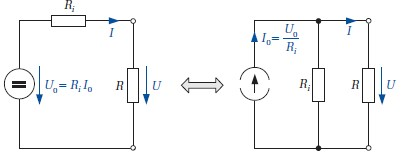
\includegraphics[width=0.7\textwidth]{Umrechnung_U_I}
%     \caption{Umrechnung}
%     \label{fig:umrechnung}
% \end{figure}



%%%%%%%%%%%%%%%%%%%%%%%%%%%%%% Einleitung - Verschiedene Spannungs- und Stromquellen %%%%%%%%%%%%%%%%%%%%%%%%%%%%%%%

\subsection{Verschiedene Spannungs- und Stromquellen}
\s{
    Die zuvor eingeführten Schaltsymbole für Spannungs- und Stromquellen sind allgemeingültig und machen keine spezifischen Aussagen 
    über die Signalform der Ausgangsgröße. Grundsätzlich wird neben der Unterscheidung zwischen Spannungs- und Stromquellen auch zwischen 
    Gleich- (DC, Direct Current) und Wechselspannung (AC, Alternating Current) differenziert.
    
    Die gebräuchlichste Form für den Betrieb elektronischer Geräte ist die Gleichspannungsquelle. Sie sorgt kontinuierlich dafür, 
    dass Ladungsträger vom Minus- zum Pluspol fließen, was ein gleichbleibendes elektrisches Feld vom Plus- zum Minuspol erzeugt.
    
    Wechselspannungsquellen (AC) hingegen haben typischerweise eine sinusförmige Ausgangsspannung bzw. einen sinusförmigen Ausgangsstrom. 
    Für den Energietransport über weite Strecken haben sich in der Vergangenheit Hochspannungsleitungen mit Wechselspannung durchgesetzt, 
    da diese technisch einfacher und kostengünstiger zu realisieren waren. Der bedeutendste Vorteil von Wechselspannung ist die einfache 
    Transformation der Spannung. Außerdem ist es praktisch, da beim Anschluss von Verbrauchern nicht auf die Verpolung geachtet werden muss.
    
    Mittlerweile gibt es jedoch auch erste Umsetzungen des Energietransports in Form von Gleichspannung. 
    Der Einsatz von Gleichstrom (DC) für lange Übertragungsstrecken, wie bei den HVDC-Leitungen (High Voltage Direct Current) 
    von der Nordsee nach Süddeutschland, bietet einige Vorteile: Gleichstrom ist effizienter, da er keine Blindleistung erzeugt, was bedeutet, 
    dass keine zusätzlichen Verluste durch die Kabelkapazität auftreten. Dadurch bleibt die Stromamplitude niedriger, 
    was zu geringeren Übertragungsverlusten führt und DC besonders für sehr lange Strecken attraktiv macht.
    In Abbildung \ref{fig:quellen} sind die Schaltzeichen der verschiedenen Quellen dargestellt. \\
}
%%%%%%%%%%%%%%%%%%%%%%%%%%%%%% Übersicht der verschiedenen Schaltzeichen von Spannungs- und Stromquellen %%%%%%%%%%%%%%%%%%%%%%%%%%%%%%%

\begin{frame}
    \ftx{Verschiedenen Spannungs- und Stromquellen}
    \b{
        \begin{figure}[h]
            \centering
            \begin{minipage}[t]{0.18\textwidth}
                \begin{circuitikz}[scale=0.9]
    \draw (0,0) to[V] (0,3)
    to[short,-o] (1.5,3)
    (0,0) to[short,-o] (1.5,0);
    \draw[-latex, thick, draw=voltage] (1.5,2.5)  to node[right, color=voltage] {$u(t)$} (1.5,0.5);
\end{circuitikz}
                \caption*{Allgemeine\\ Spannungsquelle}
            \end{minipage}
            \hfill
            \only<2->{\begin{minipage}[t]{0.18\textwidth}
                    \begin{circuitikz}[scale=0.9]
    \draw (0,0) to[dcvsource] (0,3)
    to[short,-o] (1.5,3)
    (0,0) to[short,-o] (1.5,0);
    \draw[-latex, thick, draw=voltage] (1.5,2.5)  to node[right, color=voltage] {$U$} (1.5,0.5);
\end{circuitikz}
                    \caption*{Gleichspannungsquelle}
                \end{minipage}
                \hfill
                \begin{minipage}[t]{0.18\textwidth}
                    \begin{circuitikz}[scale=0.9]
    \draw (0,0) to[vsourcesin] (0,3)
    to[short,-o] (1.5,3)
    (0,0) to[short,-o] (1.5,0);
    \draw[-latex, thick, draw=voltage] (1.5,2.5)  to node[right, color=voltage] {$u(t)$} (1.5,0.5);
\end{circuitikz}
                    \caption*{Wechselspannungsquelle}
                \end{minipage}
                \hfill
                \begin{minipage}[t]{0.18\textwidth}
                    \begin{circuitikz}[scale=0.9]
    \draw (0,0.88) -- (0,1.95);
    \draw [thick](0,0.46) circle (0.43);
    \draw (0, 0.03) -- (0,-1.05);
    \draw[-latex, thick, line width=1.1pt] (0,0.8)    to node[right] {} (0,0.1);
    \draw (0,1.95)                  to[short,-o] (1.5,1.95)
    (0,-1.05)                 to[short,-o] (1.5,-1.05);
    \draw[-latex, thick, draw=voltage] (1.5,1.45) to node[right, color=voltage] {$u(t)$} (1.5,-0.55);
\end{circuitikz}
                    \captionsetup{justification=raggedright, singlelinecheck=false}
                    \caption*{Zeitlich beliebig veränderliche Spannungsquelle}
                \end{minipage}}
            
            
            %%%%% Stromquellen
            \s{
                \vspace{0.3cm}
            }
            
            \only<3->{\begin{minipage}[t]{0.18\textwidth}
                    \begin{circuitikz}[scale=0.9]
    \draw (0,0) to[I] (0,3)
    to[short,-o] (1.5,3)
    (0,0) to[short,-o] (1.5,0)
    (0,2.4)   to[short, color=current, i_={\textcolor{current}{$i(t)$}}](0,2.5);
\end{circuitikz}
                    \caption*{Allgemeine\\ Stromquelle}
                \end{minipage}
                \hfill
                \hspace{3.9cm}
                \begin{minipage}[t]{0.18\textwidth}
                    \begin{circuitikz}[scale=0.9]
    % Zeichne den offenen Kreis
    \draw[line width=1pt] (0,-0.04) arc[start angle=10,end angle=170,radius=0.42];
    \draw[line width=1pt] (0,-0.19) arc[start angle=-10,end angle=-170,radius=0.42];

    % Zeichne die Sinuswelle in der Mitte des offenen Kreises
    \draw[thick,domain=0:360,samples=50] plot ({-0.63+1*\x/850},{0.1*sin(\x) - 0.1});

    % Anschlüsse
    \draw (-0.42,0.3) -- (-0.42,1.4) to[short, -o] (1.08,1.4)
    (-0.42,-1.6)to[short, -o] (1.08,-1.6)
    (-0.42,0.8)                to[short, color=current, i_={\textcolor{current}{$i(t)$}}]
    (-0.42,0.9);
    \draw (-0.42,-0.55) -- (-0.42,-1.6);

\end{circuitikz}
                    \captionsetup{justification=raggedright, singlelinecheck=false}
                    \caption*{Wechselstromquelle}
                \end{minipage}
                \hfill
                \begin{minipage}[t]{0.18\textwidth}
                    \begin{circuitikz}[scale=0.9]
    % Zeichne den offenen Kreis
    \draw[line width=1pt] (0,-0.04) arc[start angle=10,end angle=170,radius=0.42];
    \draw[line width=1pt] (0,-0.19) arc[start angle=-10,end angle=-170,radius=0.42];

    % Zeichne den Pfeil in der Mitte des offenen Kreises
    \draw[-latex, thick, line width=1.1pt] (-0.42,-0.45)    to node[right] {} (-0.42,0.25);

    % Anschlüsse
    \draw (-0.42,0.3) -- (-0.42,1.4) to[short, -o] (1.08,1.4)
    (-0.42,-1.6)to[short, -o] (1.08,-1.6)
    (-0.42,0.8)                to[short, color=current, i_={\textcolor{current}{$i(t)$}}]
    (-0.42,0.9);
    \draw (-0.42,-0.55) -- (-0.42,-1.6);

\end{circuitikz}
                    \captionsetup{justification=raggedright, singlelinecheck=false}
                    \caption*{Zeitlich beliebig veränderliche Stromquelle}
                \end{minipage}}
            
        \end{figure}
    }% nur Folie
    
    \speech{02_Spannungs_und_Stromquellen}{12}{ % ToDo: only 1
        Wir haben bisher das Symbol kennengelernt für eine allgemeine Spannungsquelle. 
        Das heißt, bei diesem Symbol, was Sie hier sehen, ein Kreis, durch den senkrecht ein Strich geht, 
        das bezeichnet eine allgemeine Spannungsquelle. 
        Mit diesem Symbol wird nicht gesagt, welche Form die Spannung hat. 
        Ob es sich um eine Gleichspannung, eine Wechselspannung oder eine zeitlich veränderliche Spannung handelt, 
        das kann alles sein.    
    }
    
    \speech{02_Spannungs_und_Stromquellen}{13}{ % ToDo: only 2 - 4
        Da wir aber sehr häufig Gleich- und Wechselspannungskreise haben, gibt es auch hierfür gesonderte Symbole. 
        Die Gleichspannungsquelle ist ein Kreis mit zwei sich seitlich überstehenden Platten. 
        Das soll zum Beispiel einen Kondensator, eine Anode oder eine Batterie symbolisieren. 
        Bei der Wechselspannung schreiben wir die Spannungsform direkt ins Symbol: 
        Wir haben dort eine zeitlich variable Spannung, die einem Sinus oder Kosinus folgt, 
        Näheres dazu in den entsprechenden Modulen. 
        Und dann gibt es noch die zeitlich beliebig veränderliche Spannungsquelle, 
        dargestellt durch einen Kreis mit einem Pfeil.    
    }
    
    \speech{02_Spannungs_und_Stromquellen}{14}{ % ToDo: only 5 - 7
        Für die Stromquelle gilt das Gleiche. 
        Wir haben bisher, unten links dargestellt, die allgemeine Stromquelle verwendet. 
        Das ist ein Kreis mit einem waagrechten Strich darin. 
        Und genauso gibt es eine Wechselstromquelle und eine zeitlich veränderliche Stromquelle.
        Ein eigenes Symbol für die Gleichstromquelle gibt es in dieser Darstellung nicht.
        
        Wenn wir uns die allgemeinen Darstellungen der Spannungs- und Stromquelle noch einmal anschauen, 
        fällt auf, dass sie sich sehr ähnlich sind: 
        Beide haben den Kreis, und in einem Fall einen senkrechten, im anderen einen waagrechten Strich.
        
        Diese Symbolik hilft uns tatsächlich auch dabei zu erkennen, 
        wie man eine zu Null gesetzte Quelle in einer Schaltung ersetzen kann. 
        Wenn wir also z.B. eine Spannungsquelle auf Null setzen wollen, was wir in manchen Berechnungen tun, 
        dann müssen wir sicherstellen, dass dort garantiert eine Spannung von Null Volt anliegt. 
        Und bei welcher Verschaltung ist das gegeben? 
        Bei einem Kurzschluss. An einem Kurzschluss fällt eine Spannung von 0 Volt ab. 
        Und wenn wir aus dem Symbol der allgemeinen Spannungsquelle den Kreis weglassen, 
        bleibt ein einfacher Strich übrig, wie ein Kurzschluss.
        
        Für die Stromquelle ist das analog: 
        Wenn wir sie auf Null setzen wollen, darf kein Strom mehr fließen. 
        Das erreichen wir durch einen Leerlauf. Auch hier, wenn man den Kreis weglässt, 
        sieht das Symbol wie ein Leerlauf aus: zwei nicht verbundene Anschlüsse, zwischen denen kein Strom fließen kann.
        
        Das ist eine hilfreiche Merkhilfe für spätere Berechnungen in diesem und in folgenden Modulen.
    }
    
\end{frame}

\s{
    \begin{figure}[h]
        \centering
        \begin{minipage}[t]{0.18\textwidth}
            \begin{circuitikz}[scale=0.9]
    \draw (0,0) to[V] (0,3)
    to[short,-o] (1.5,3)
    (0,0) to[short,-o] (1.5,0);
    \draw[-latex, thick, draw=voltage] (1.5,2.5)  to node[right, color=voltage] {$u(t)$} (1.5,0.5);
\end{circuitikz}
            \caption*{Allgemeine\\ Spannungsquelle}
        \end{minipage}
        \hfill
        \begin{minipage}[t]{0.18\textwidth}
            \begin{circuitikz}[scale=0.9]
    \draw (0,0) to[dcvsource] (0,3)
    to[short,-o] (1.5,3)
    (0,0) to[short,-o] (1.5,0);
    \draw[-latex, thick, draw=voltage] (1.5,2.5)  to node[right, color=voltage] {$U$} (1.5,0.5);
\end{circuitikz}
            \caption*{Gleichspannungsquelle}
        \end{minipage}
        \hfill
        \begin{minipage}[t]{0.18\textwidth}
            \begin{circuitikz}[scale=0.9]
    \draw (0,0) to[vsourcesin] (0,3)
    to[short,-o] (1.5,3)
    (0,0) to[short,-o] (1.5,0);
    \draw[-latex, thick, draw=voltage] (1.5,2.5)  to node[right, color=voltage] {$u(t)$} (1.5,0.5);
\end{circuitikz}
            \caption*{Wechselspannungsquelle}
        \end{minipage}
        \hfill
        \begin{minipage}[t]{0.18\textwidth}
            \begin{circuitikz}[scale=0.9]
    \draw (0,0.88) -- (0,1.95);
    \draw [thick](0,0.46) circle (0.43);
    \draw (0, 0.03) -- (0,-1.05);
    \draw[-latex, thick, line width=1.1pt] (0,0.8)    to node[right] {} (0,0.1);
    \draw (0,1.95)                  to[short,-o] (1.5,1.95)
    (0,-1.05)                 to[short,-o] (1.5,-1.05);
    \draw[-latex, thick, draw=voltage] (1.5,1.45) to node[right, color=voltage] {$u(t)$} (1.5,-0.55);
\end{circuitikz}
            \captionsetup{justification=raggedright, singlelinecheck=false}
            \caption*{Zeitlich beliebig veränderliche Spannungsquelle}
        \end{minipage}
        
        
        %%%%% Stromquellen
        
        \vspace{0.3cm}
        
        
        \begin{minipage}[t]{0.18\textwidth}
            \begin{circuitikz}[scale=0.9]
    \draw (0,0) to[I] (0,3)
    to[short,-o] (1.5,3)
    (0,0) to[short,-o] (1.5,0)
    (0,2.4)   to[short, color=current, i_={\textcolor{current}{$i(t)$}}](0,2.5);
\end{circuitikz}
            \caption*{Allgemeine\\ Stromquelle}
        \end{minipage}
        \hfill
        \hspace{4.2cm}
        \begin{minipage}[t]{0.18\textwidth}
            \begin{circuitikz}[scale=0.9]
    % Zeichne den offenen Kreis
    \draw[line width=1pt] (0,-0.04) arc[start angle=10,end angle=170,radius=0.42];
    \draw[line width=1pt] (0,-0.19) arc[start angle=-10,end angle=-170,radius=0.42];

    % Zeichne die Sinuswelle in der Mitte des offenen Kreises
    \draw[thick,domain=0:360,samples=50] plot ({-0.63+1*\x/850},{0.1*sin(\x) - 0.1});

    % Anschlüsse
    \draw (-0.42,0.3) -- (-0.42,1.4) to[short, -o] (1.08,1.4)
    (-0.42,-1.6)to[short, -o] (1.08,-1.6)
    (-0.42,0.8)                to[short, color=current, i_={\textcolor{current}{$i(t)$}}]
    (-0.42,0.9);
    \draw (-0.42,-0.55) -- (-0.42,-1.6);

\end{circuitikz}
            \captionsetup{justification=raggedright, singlelinecheck=false}
            \caption*{Wechselstromquelle}
        \end{minipage}
        \hfill
        \begin{minipage}[t]{0.18\textwidth}
            \begin{circuitikz}[scale=0.9]
    % Zeichne den offenen Kreis
    \draw[line width=1pt] (0,-0.04) arc[start angle=10,end angle=170,radius=0.42];
    \draw[line width=1pt] (0,-0.19) arc[start angle=-10,end angle=-170,radius=0.42];

    % Zeichne den Pfeil in der Mitte des offenen Kreises
    \draw[-latex, thick, line width=1.1pt] (-0.42,-0.45)    to node[right] {} (-0.42,0.25);

    % Anschlüsse
    \draw (-0.42,0.3) -- (-0.42,1.4) to[short, -o] (1.08,1.4)
    (-0.42,-1.6)to[short, -o] (1.08,-1.6)
    (-0.42,0.8)                to[short, color=current, i_={\textcolor{current}{$i(t)$}}]
    (-0.42,0.9);
    \draw (-0.42,-0.55) -- (-0.42,-1.6);

\end{circuitikz}
            \captionsetup{justification=raggedright, singlelinecheck=false}
            \caption*{Zeitlich beliebig veränderliche Stromquelle}
        \end{minipage}
        
        \caption{\textbf{Verschiedene Spannungs- und Stromquellen.}}
        \label{fig:quellen}
    \end{figure}
}


%%%%%%%%%%%%%%%%%%%%%%%%%%%%%% Ende %% Übersicht der verschiedenen Schaltzeichen von Spannungs- und Stromquellen %%%%%%%%%%%%%%%%%%%%%%%%%%%%%%%

%%%%%%%%%%%%%%%%%%%%%%%%%%%%% Bemerkung zu den Quellen %%%%%%%%%%%%%%%%%%%%%%%%%%%%%%%%%%%%%%%%%%%%%%%%%
\s{
    Es ist zu berücksichtigen, dass Wechselspannungs- und Stromquellen eine sinusförmige Ausgangsspannung bzw. einen sinusförmigen Ausgangsstrom haben, 
    wohingegen die zeitlich beliebig veränderlichen Quellen jede beliebige Form haben können.
    Ein Beispiel dafür ist das Rechtecksignal, welches aus dem Ein- und Ausschalten einer Gleichspannungsquelle stammen könnte.
    Genutzt werden solche Quellen beispielsweise in der mobilen Anwendung der weit verbreiteten Bauart von Elektromotoren, welche auch Synchron, bzw. Asynchronmaschinen genannt werden.
    Diese Motoren werden in mobilen Anwendungen durch eine Gleichspannungsquelle betrieben, dessen Signalform mithilfe einer Leistungselektronik in das gewünschte Rechtecksignal gewandeln (gepulst) werden
    und im Motor durch über die Spulenwicklungen aus dem gepulsten Spannungssignal ein sinusförmigen Strom entsteht. Mehr dazu im Modul elektrische Maschinen.
    Ein weiteres Beispiel für zeitlich beliebige Signale ist die digitale Informationsübertragung in der Nachrichtentechnik, wobei eine Eins dem Highsignal und eine Null einem Lowsignal entspricht,
    was ebenfalls einem Rechtecksignal gleicht.
}
%%%%%%%%%%%%%%%%%%%%%%%%%%%%% Ende - Bemerkung zu den Quellen %%%%%%%%%%%%%%%%%%%%%%%%%%%%%%%%%%%%%%%%%%%%%%%%%



